\documentclass{beamer}

\usepackage{beamerthemesplit}
\usetheme{CambridgeUS}
\usepackage{ucs}
\usepackage[czech]{babel}
\usepackage[utf8]{inputenc}
\usepackage{palatino}
\usepackage{graphicx}

\title{ITY -- 5. projekt}
\subtitle{Grafové algoritmy -- BFS}
\author{Radek Švec (xsvecr01)}
\institute[VUT FIT]{Vysoké učení technické v Brně \\
                    Fakulta informačních technologií}
\date{\today}

\begin{document}

\begin{frame}
  \titlepage
\end{frame}

\begin{frame}{Obsah prezentace}
    \setbeamertemplate{section in toc}[sections numbered]
	\tableofcontents[hideallsubsections]
\end{frame}

\section{Co je Breadth-First Search}
\begin{frame}{Co je Breadth-First Search}
	\begin{itemize}
		\item
		Breadth-First Search (\alert{BFS}) je algoritmus \textbf{prohledávání grafu do šířky}.
		\item
			Princip:
			\begin{itemize}
				\item Algoritmus nejprve prochází všechny sousedy startovního vrcholu, pak sousedy sousedů atd..
				\item Funguje na způsob \alert{FIFO} fronty. (První uzel, který je do fronty vložen je jako první zpracován.)
			\end{itemize}
	\end{itemize}
\end{frame}

\section{Ukázka algoritmu}
\begin{frame}{Příklad}
    Projděte graf pomocí BFS
    \begin{center}
      \onslide<1>\centering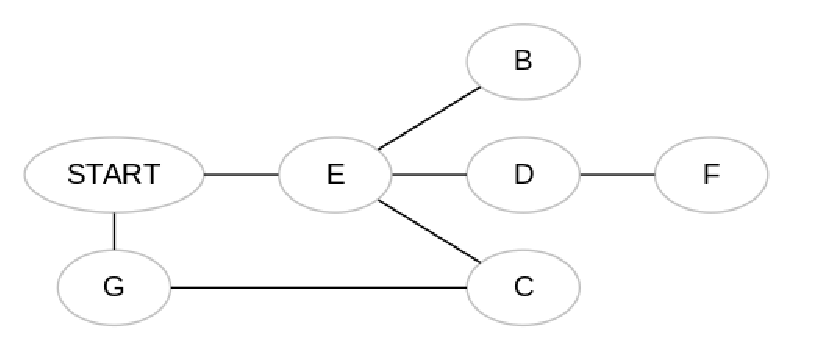
\includegraphics[width=0.7\textwidth]{./img/1.eps}
    \end{center}
\end{frame}

\begin{frame}{Postup algoritmu}
    \begin{center}
        \begin{tabular}{ c l l }
             Krok & Fronta(první prvek vlevo) & Zpracované uzly \\ 
             1 & START & -- \\  
             2 & E, G & START \\   
             3 & G, B, C, D & START, E \\  
             4 & B, C, D & START, E, G \\  
             5 & C, D & START, E, G, B \\  
             6 & D & START, E, G, B, C \\  
             7 & F & START, E, G, B, C, D \\  
             8 & -- & \alert{START, E, G, B, C, D ,F} \\  
        \end{tabular}
    \end{center}
\end{frame}

\begin{frame}{Grafické zobrazení}
	\begin{figure}
    \begin{overprint}
    \onslide<1>\centering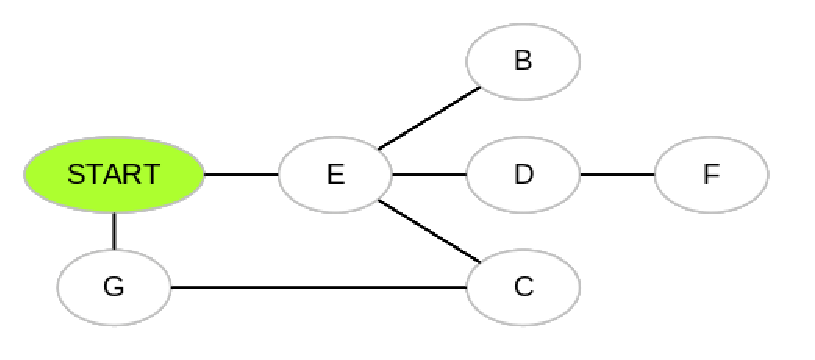
\includegraphics[width=0.7\textwidth]{./img/2.eps}
    \onslide<2>\centering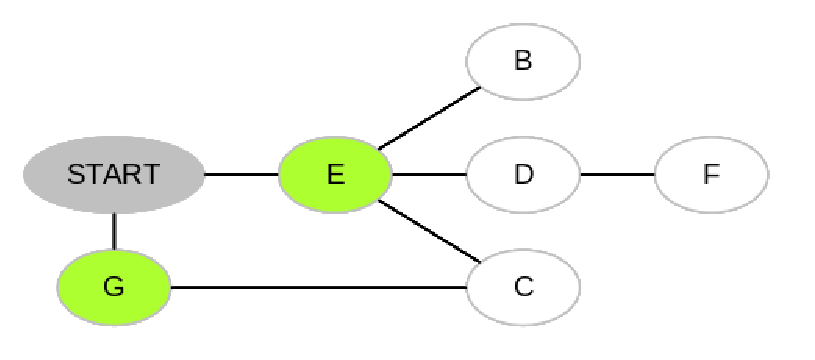
\includegraphics[width=0.7\textwidth]{./img/3.eps}
    \onslide<3>\centering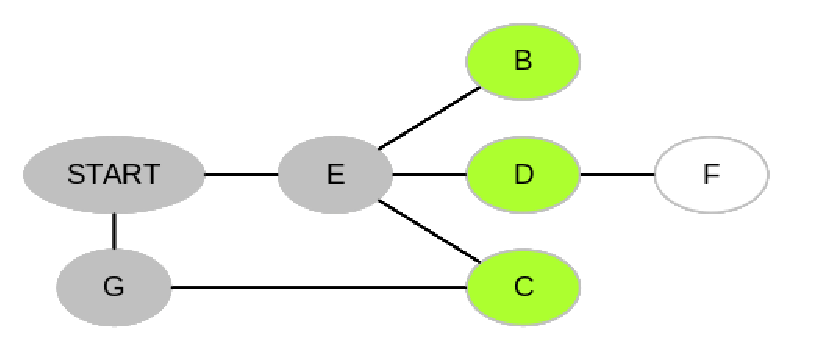
\includegraphics[width=0.7\textwidth]{./img/4.eps}
    \onslide<4>\centering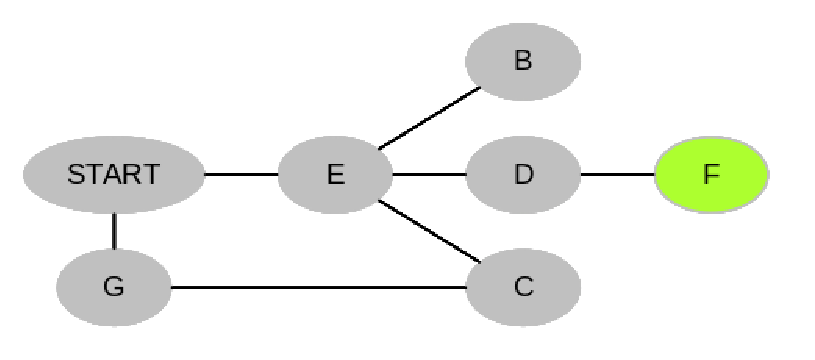
\includegraphics[width=0.7\textwidth]{./img/5.eps}
    \onslide<5>\centering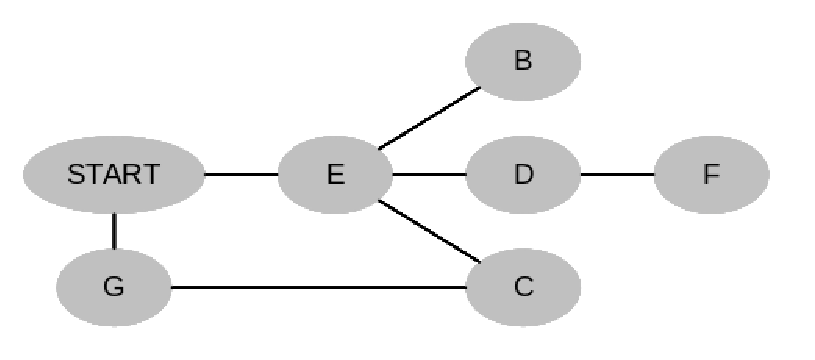
\includegraphics[width=0.7\textwidth]{./img/6.eps}
    \end{overprint}
\end{figure}
\end{frame}

\section{Pseudokód algoritmu}
\begin{frame}[fragile]{Pseudokód algoritmu}
    \fontsize{10pt}{7.2}\selectfont
    \begin{semiverbatim}
 1 void BFS (Graph G, Node s) \{   
 2   for (Node u in U(G)-s)
 3     \{ state[u] = FRESH; d[u] = infinity; p[u] = null; \}
 4   state[s] = OPEN; d[s] = 0; p[s] = null;
 5   Queue.Init();
 6   Queue.Push(s);
 7   while (!Queue.Empty()) \{
 8     u = Queue.Pop();
 9     for (v in Adj[u]) \{
10       if (state[v] == FRESH) \{
11         state[v] = OPEN;
12         d[v] = d[u]+1;
13         p[v] = u;
14         Queue.Push(v); 
15       \}
16     \}
17     state[u]=CLOSED;
18   \}
19 \}
    \end{semiverbatim}
\end{frame}

\section{Složitost algoritmu}
\begin{frame}{Složitost algoritmu}
	\begin{itemize}
		\item
		Asymptotická složitost algoritmu je \alert{$O(V + E)$}, kde:
		\begin{itemize}
		    \item 
		    $V$ je počet uzlů
		    \item
		    a $E$ je počet hran
		\end{itemize}
		\item
		\textbf{Složitost je tedy \alert{lineární}}
	\end{itemize}
\end{frame}

\section*{}
\begin{frame}{Děkuji za pozornost}
	Prostor pro Vaše dotazy.
\end{frame}

\end{document} 